% ---------------------------------------------------
\chapter{``¡Hola, Mundo!'' en Rust}
\label{ch_hola_mundo}
% ---------------------------------------------------
\IndiceCapitulo

\begin{Resumen}
Para poder seguir el contenido del curso es importante tener instalado el entorno de desarrollo del lenguaje Rust. La instalación es sencilla y rápida, si se siguen las instrucciones que se dan en la propia página del proyecto y que se indicarán en este primer capítulo de la documentación del curso. 

\smallskip

Además, es importante utilizar un editor de texto con los complementos necesarios para trabajar con Rust. Los contenidos del curso se han desarrollado utilizando Visual Studio Code de Micrososft y RustRover de Jet Brians. Ambos son editores de gran calidad y que ofrecen importantes ayudas a la programación en Rust.

\smallskip

Esté capítulo de la documentación del curso se completa con la explicación de cómo desarrollar el clásico programa ``¡Hola, Mundo!'' y con la explicación de algunos conceptos comunes, como la inclusión de comentarios en el código, la utilización de algunas macros del lenguaje útiles en entornos de depuración y pruebas y la posible utilización del portal ``Rust Playground''.
\end{Resumen}

\section{Instalación de Rust}

Para instalar el entorno de desarrollo de Rust, el método más sencillo es descargarse el \textit{script} de instalación que se proporciona para cada sistema operativo y ejecutarlo en el ordenador. Las instrucciones se dan en la página Web de Rust, en la siguiente dirección:

{\centering \small \texttt{https://www.rust-lang.org/tools/install} \par}

Los usuarios de Linux y de Mac no tendrán problema en seguir las instrucciones que se dan en dicha página. Los usuarios de Windows pueden descargar el instalador directamente del siguiente enlace:

{\centering \footnotesize \texttt{https://static.rust-lang.org/rustup/dist/i686-pc-windows-gnu/rustup-init.exe} \par}

Para poder compilar y construir los programas se necesita un \textit{linker}. Es posible que ya lo tenga instalado en su sistema. Si aparecieran errores relativos a la falta del \textit{linker}, hay que instalar un compilador de \texttt{C}, que suele tener el \textit{linker} ya incorporado. En cualquier caso, es útil tener un compilador de \texttt{C} instalado en el sistema, pues algunos paquetes pueden depender de él para su correcto funcionamiento.

Los usuarios de \textit{Linux} pueden instalar \texttt{GCC} o \texttt{Clang}, el que sea acorde a su distribución. Los usuarios de \textit{Ubuntu} pueden instalar el paquete \texttt{build-essentials}.

Los usuarios de \textit{macOS} pueden obtener un compilador de \texttt{C}
tecleando la siguiente instrucción:

{\centering \texttt{xcode-select --install}\par}

Los usuarios de \textit{Windows} deben seguir las instrucciones de instalación que se dan en la página web del proyecto Rust \citep{klabnikRustProgrammingLanguage}, en la siguiente dirección web:

{\centering\fontfamily{lmss}\selectfont{https://www.rust-lang.org/tools/install}\par}

Durante la instalación, se le indicará al usuario que necesita tener instaladas las herramientas de \texttt{C++} para \textit{Visual Studio 2013} o posterior. Se pueden instalar las herramientas para \textit{Visual Studio 2019} comprobando que se activa la opción correspondiente a la instalación de las \textit{C++ build tools}, el \textit{SDK} para \textit{Windows 10} y los componentes en inglés de dicho \textit{pack}.

La instalación que hace \texttt{rustup} incluye el programa \texttt{rustup}, el compilador \texttt{rustc} y el gestor de paquetes \textit{Cargo}. Para comprobar que el conjunto de desarrollo está correctamente instalado en el ordenador, se pueden probar las siguientes ordenes en la consola:

\begin{Codigo}
rustup show
rustc --version
cargo --version
\end{Codigo}

El resultado debería ser similar al de la Figura \ref{fig_rustup}.

\begin{figure}[H]
   \begin{center}
      \setlength\fboxsep{2pt}
      \setlength\fboxrule{0.5pt}
      \fbox{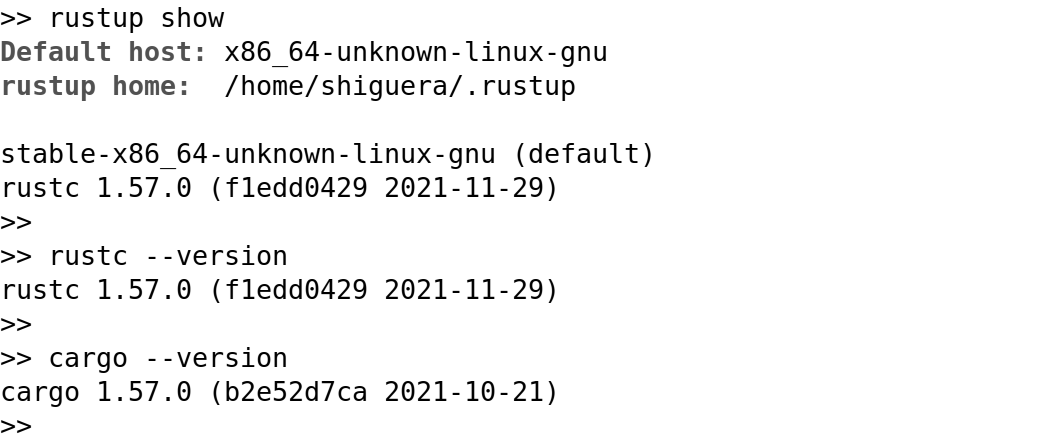
\includegraphics[width=0.9\textwidth]{img/figura_rustup_bw.png}}
      \caption{Instrucciones en el terminal para comprobar las versiones instaladas de los programas \textit{rustup}, \textit{rustc} y \textit{cargo}}
      \label{fig_rustup}
   \end{center}
\end{figure}

Si no aparecen los mensajes y se está trabajando en \textit{Windows}, debería comprobar que Rust está en la variable \texttt{\%PATH\%} del sistema. En adelante, las instrucciones que se indican en este libro deberían de funcionar en los terminales de cualquiera de los tres sistemas operativos.

Para actualizar a una versión más reciente de Rust, hay que teclear en el terminal la siguiente instrucción:

{\centering\texttt{rustup update}\par}

Para desinstalar Rust hay que teclear:

{\centering\texttt{rustup self uninstall}\par}

Al instalar Rust, se carga en el ordenador una versión de la documentación. Mediante la siguiente instrucción, se puede consultar dicha documentación localmente en el navegador:

{\centering\texttt{rustup doc}\par}

Podrá navegar a través de multitud de documentos y libros que le servirán para profundizar sobre Rust. En particular, un buen comienzo es el ``Libro de Rust'', escrito y mantenido por Steve Klabnik y Carol Nichols, con contribuciones de la \textit{Rust Community}. Además de la copia que se instala en su ordenador, puede consultar la versión más actualizada en la web, en la referencia \citep{klabnikRustProgrammingLanguage}:

{\centering \small \texttt{https://doc.rust-lang.org/book/} \par}

El portal oficial de Rust ofrece enlaces a diversos documentos de interés en la siguiente dirección:

{\centering \small \texttt{https://www.rust-lang.org/learn} \par}

Cuando le surjan dudas acerca de alguna función o instrucción de las que se explican en este libro, la mejor manera de acceder a una documentación más completa de la misma es la referencia de la API de la librería estándar. La documentación local le ofrecerá una copia, o también la puede 
consultar en la web en la referencia \citep{rustfoundationRustStandardLibrary}.

A día de hoy, existen numerosos libros donde iniciarse o profundizar en los distintos aspectos del lenguaje. Como no podía ser de otra manera, el autor de estas líneas considera que su libro ``Programación en Rust'', publicado en la Editorial Garceta, es una buena herramienta para aprender a programar en Rust \citep{higueradefrutosProgramacionRust2022}.

Otras editoriales que disponen de libros sobre Rust son:
\begin{itemize}
   \item \textit{Packt}: {\small \texttt{https://www.packtpub.com/}}
   \item \textit{Manning}: {\small \texttt{https://www.manning.com/}}
   \item \textit{O'Reilly}: {\small \texttt{https://www.oreilly.com/}}
\end{itemize}

\subsection{El editor de texto}

\noindent Para completar el entorno de trabajo, será necesario disponer de un editor. El código de los programas en lenguaje Rust se escribe en ficheros de texto plano. Se puede utilizar cualquier editor de texto para ello. En el siguiente enlace se muestran los editores que están comprobados por la fundación Rust y que proporcionan herramientas de compilación integradas, ayudas y corrección de sintaxis y otras:

{\centering \small \texttt{https://www.rust-lang.org/tools} \par}

El autor utiliza habitualmente Visual Studio Code de Microsoft y RustRover de JetBrains. 

\textit{Visual Studio Code} de \textit{Microsoft} \citep{VisualStudioCode}, es una buena opción. Hay versiones para cualquier sistema operativo, es gratuito, de buena calidad y dispone de una buena integración con Rust. El nombre con el que se suele denominar al
programa es \textit{VS Code}.

Para sacar el máximo provecho de la utilización de \textit{VS Code} al programar en Rust, es conveniente instalar la extensión existente para Rust, que ofrece numerosas ayudas, como autocompletado, remarcado de errores, terminal para ejecutar las órdenes de compilación\footnote{En la opción del menú \texttt{View::Terminal}, el programa  \textit{VS Code} ofrece un terminal para ejecutar todos los comandos. En el caso de los usuarios de \textit{Windows}, el terminal ofrecido es \textit{Power Shell}, aunque se puede configurar para utilizar el terminal \texttt{cmd} estándar.}, gestión de paquetes
y otras utilidades que facilitan mucho la gestión de los programas en Rust. Se puede consultar cómo hacerlo en:

{\centering \small \texttt{https://code.visualstudio.com/docs/languages/rust} \par}

\textit{RustRover} está desarrollado por JetBrains. JetBrains dispone de editores de gran calidad para varios lenguajes. Son de pago, pero ofrece versiones completas de manera gratuita para estudiantes y profesores. Utilizando una cuenta de correo de la UPM, se puede disfrutar de dichas ventajas en todos los editores de JetBrains. El editor RustRover se puede desacargar desde la siguiente dirección:

{\centering \small \texttt{https://www.jetbrains.com/rust/} \par}

Los dos editores comentados son de gran calidad y también lo serán, con seguridad, el resto de editores recomendados por la Fundación Rust, aunque el autor no ha tenido ocasión de probarlos.

\pagebreak

\section{¡Hola, mundo! en Rust}
\noindent Siguiendo la tradición, se va a explicar cómo crear el primer programa en Rust, un programa que imprima \texttt{¡Hola, mundo!} en el terminal del ordenador. Se supone que se está trabajando en el terminal del sistema. Se recomienda crear un directorio para los programas escritos en Rust y, dentro de él, directorios individuales para cada programa. Para este primer programa, la forma de proceder en \textit{Linux, macOS} o \textit{Windows} con \textit{Power Shell} podría ser la siguiente:
\begin{Codigo}
mkdir ~/rust_projets
cd ~/rust_projects
mkdir hola_mundo
cd hola_mundo
\end{Codigo}

En el caso de estar trabajando en la terminal \texttt{cmd} de \textit{Windows}, las instrucciones equivalentes serían las siguientes:
\begin{Codigo}
mkdir "%USERPROFILE%\rust_projects"
cd /d "%USERPROFILE%\rust_projects"
mkdir hola_mundo
cd hola_mundo
\end{Codigo}

Con ello, se ha creado un directorio llamado \texttt{rust\_projects} en el directorio del usuario y, dentro de él, un directorio llamado \texttt{hola\_mundo}. Tras crear los directorios, nos hemos posicionado dentro del directorio \texttt{hola\_mundo}. Obsérvese que, para el nombre de los directorios del proyecto, se ha utilizado lo que será el convenio habitual para nombrar programas, variables y funciones en el lenguaje Rust, el denominado \textit{snake case}: letras minúsculas separando las palabras con el guión bajo.

A continuación, utilizando el editor de texto, cree un fichero llamado \texttt{main.rs} para teclear el código del programa. Los ficheros de código en Rust tienen la extensión \texttt{rs}. Se podría llamar al fichero con otro nombre, pero también es convenio que el programa que contiene la función \texttt{main()} se llame \texttt{main.rs}. Esta función  es lo primero que se ejecuta en los programas escritos en Rust. Teclee el siguiente código en la función recién creada:

\begin{Codigo}
fn main() {
   println!("¡Hola, mundo!");
}
\end{Codigo}

La primera línea es la signatura\footnote{En teoría de programación, se denomina \textit{signatura} de una función a la primera línea, en la que se declara el nombre, los parámetros y el valor devuelto por la función.} de la función \textit{main()}. Como se puede observar, consta de la palabra clave \textit{fn},
que indica al compilador que se está declarando una función, seguida por el nombre de la función, en este caso \textit{main}. A continuación se escriben dos paréntesis, en esta ocasión vacíos. Dentro de estos paréntesis se escriben los parámetros que admite la función. En este caso, la función \textit{main()} no recibe ningún parámetro. A continuación, se pondría el tipo de datos del valor devuelto por la función, pero en este caso la función \textit{main()} tampoco devuelve ningún valor.

A continuación se escribe el código de la función, encerrado entre una pareja de llaves \texttt{\{\}}. El convenio de escritura en Rust es escribir la llave de apertura en la línea de signatura; las instrucciones que componen el cuerpo de la función se escriben en las lineas siguientes, tabuladas hacia la derecha; finalmente, la llave de cierre de la función se escribe en una línea nueva tras la última instrucción, alineada con la palabra \texttt{fn} de la signatura.

Al instalar Rust, se instala también la utilidad \texttt{rustfmt} que permite formatear los ficheros de código fuente siguiendo los convenios de escritura de Rust. Para ello, solo hay que teclear en el terminal la orden siguiente:

{\centering\texttt{rustfmt nombre\_del\_fichero\_fuente}\par}

El código de la función \texttt{main()} recién creada consta de una sola línea. Se trata de la macro \texttt{println!()} que escribe una línea de texto en la pantalla. En este caso se le ordena escribir la cadena de caracteres \texttt{"¡Hola, mundo!"}. Se hablará algo más de la macro \texttt{println!()} en el Apartado \ref{sec_codigo_ejemplos}.

Para poder ejecutar el programa hay que compilarlo. Esto se consigue tecleando la siguiente instrucción en el terminal:

\vspace{0.2em}
{\centering\texttt{rustc main.rs}\par}

El programa \texttt{rustc} es el compilador de Rust. Al ejecutar la instrucción anterior, se compila el programa y se crea un ejecutable, llamado \texttt{main}. 

\pagebreak

Si tras esa instrucción se listan los ficheros del directorio, se ve que hay un fichero ejecutable \texttt{main}. En \textit{Windows}, el ejecutable se llama \texttt{main.exe} y además, se crea otro fichero llamado \texttt{main.pdb} que contiene instrucciones internas de compilación.

Para ejecutar el programa, en \textit{Linux} y \textit{macOS} hay que teclear la siguiente instrucción:

\vspace{0.2em}
{\centering\texttt{./main}\par}

\vspace{0.2em}
En el terminal \texttt{cmd} de \textit{Windows}, la instrucción sería:

{\centering\texttt{.\textbackslash main.exe}\par}

En ambos casos, se obtendrá en pantalla la frase:

{\centering\texttt{¡Hola, mundo!}\par}

%\vspace{0.2em}
\section{¡Hola, mundo!, utilizando Cargo}
\label{sec_cargo}
\noindent El proceso descrito en el apartado anterior, consistente en compilar directamente con \texttt{rustc} el fichero fuente, puede servir para programas que constan de un solo fichero fuente. Pero, en general, los programas constarán de más de un fichero fuente y es conveniente organizar el código de todos los ficheros y el proceso de compilación de manera eficiente.

Una de las utilidades que queda instalada en el ordenador con Rust es el gestor de paquetes \textit{Cargo}. Se trata de un gestor de paquetes muy completo que facilita mucho la tarea de creación y mantenimiento de los programas escritos en lenguaje Rust.

El gestor \textit{Cargo} se encarga de construir y compilar los programas. También se encarga de gestionar las \textit{dependencias} de los proyectos. En Rust, se denominan \textit{dependencias} las librerías externas que se deban incorporar al programa. Una vez definidas las dependencias del proyecto, \textit{Cargo} se encarga de descargarlas,  mantenerlas actualizadas y compilarlas. Existen miles de librerías disponibles para Rust. Puede consultarlas en el repositorio público ``The Rust community’s crate registry'' \citep{communityofrustdevelopersRustCommunityCrate}.

Se va a realizar ahora un programa tipo ``\textit{Hola Mundo}'', similar al realizado en el apartado anterior, pero utilizando el gestor de paquetes \textit{Cargo}. Para ello, desde el terminal, sitúese en el directorio que creó para albergar los proyectos de Rust y teclee la siguiente instrucción:

{\centering\texttt{cargo new hola\_cargo}\par}

Con esta instrucción, el programa \textit{Cargo} creará una nueva carpeta de nombre \texttt{hola\_cargo} y, dentro de ella, varias carpetas y archivos que constituyen un programa ejecutable. Si se sitúa dentro de la carpeta del proyecto recién creado y lista los archivos y carpetas creados por \textit{Cargo} al crear el programa, obtendrá un resultado similar al de la Figura \ref{fig_holacargo}.

\begin{figure}[H]
   \begin{center}
      \setlength\fboxsep{2pt}
      \setlength\fboxrule{0.5pt}
      \fbox{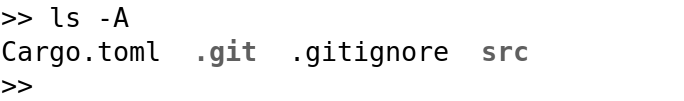
\includegraphics[width=0.5\textwidth]{img/figura_holacargo_bw.png}}
      \caption{Ficheros y carpetas creados en el directorio del proyecto \textit{hola\_cargo}, tras su creación por \textit{Cargo}}
      \label{fig_holacargo}
   \end{center}
\end{figure}

En la Figura \ref{fig_holacargo} se puede ver que se ha creado el fichero \texttt{Cargo.toml} \footnote{TOML es el acrónimo de <<\textit{Tom's Obvious, Minimal Language}>>. Este lenguaje está pensado para los ficheros de configuración. Su creador fue \textit{Tom Preston-Werner}.}. Este fichero contiene la información necesaria para compilar el programa. También se incluirían ahí las dependencias, si las hubiera. El contenido de dicho fichero, en el proyecto recién creado es similar al siguiente:
\begin{Codigo}
[package]
name = "hola_cargo"
version = "0.1.0"
edition = "2021"

# See more keys and their definitions at
# https://doc.rust-lang.org/cargo/reference/manifest.html

[dependencies]
\end{Codigo}

Las secciones de este fichero comienzan con un nombre de sección entre corchetes. La primera sección, \texttt{[package]}, contiene el nombre y la versión del programa y la edición de Rust utilizada para su creación. A continuación hay unos comentarios, que son las líneas que comienzan con el carácter \#. Finalmente, hay una sección \texttt{[dependencies]} inicialmente vacía.

Además del fichero \texttt{Cargo.toml}, en la carpeta del proyecto recién creado aparece un fichero \texttt{.gitignore} y una carpeta \texttt{.git}. Al crear un nuevo programa, \textit{Cargo} inicializa un repositorio \textit{GIT} para el mismo. Se pueden utilizar también otros gestores de versiones.

También se puede crear un nuevo proyecto Rust en un directorio donde ya exista un repositorio \textit{GIT}, mediante la orden \texttt{cargo init}. Puede teclear en la consola la orden \texttt{cargo new --help} para obtener más información o consultar el <<Libro de Cargo>> \citep{CargoBook} en la
documentación de Rust.

En el directorio del proyecto hay un directorio llamado \texttt{src} y, dentro de él, un fichero llamado \texttt{main.rs}. Si edita el fichero \texttt{main.rs} verá que contiene un código como el siguiente:
\begin{Codigo}
fn main() {
   println!("Hello, world!");
}
\end{Codigo}

Es la función \texttt{main()} con la misma instrucción \texttt{println!()} que se utilizó en el apartado anterior. Cada vez que \textit{Cargo} crea un nuevo programa, lo crea como un programa <<\textit{Hola Mundo}>> listo para funcionar.

Para compilar y ejecutar el programa hay que teclear en el terminal la siguiente instrucción:

{\centering\texttt{cargo run}\par}

Si vuelve a listar el directorio del proyecto verá que se ha creado una nueva carpeta llamada \texttt{target}. Dentro de ella hay otras carpetas y ficheros. El ejecutable creado está en la carpeta \texttt{target/debug} y lo podrá ejecutar en \textit{Linux} y \textit{macOS} con la instrucción siguiente:

{\centering\texttt{./target/debug/hola\_cargo}\par}

En \textit{Windows}, la instrucción que hay que teclear para ejecutar el programa es:

{\centering\texttt{.\textbackslash target\textbackslash debug\textbackslash hola\_cargo.exe}\par}

En el directorio del proyecto verá que también se ha creado un fichero \texttt{Cargo.lock}. Se trata de un fichero que utiliza el programa \textit{Cargo} para gestionar las versiones utilizadas de las dependencias. Dicho fichero lo mantiene de manera automática el programa \textit{Cargo} y el usuario no necesita modificarlo. Si tiene curiosidad, puede listar el fichero para ver su contenido.

Se puede compilar o construir el programa sin ejecutarlo, mediante la siguiente instrucción:

{\centering\texttt{cargo build}\par}

El comando \texttt{cargo build} admite diferentes opciones de compilación en combinación con las especificaciones del fichero \texttt{Cargo.toml}. Tienen que ver con la versión a construir, la realización de test y otras. Se recomienda consultar el ``\textit{Libro de Cargo}'' \citep{CargoBook} para ampliar la información al respecto.

A veces, la primera vez que se construye el programa o tras varias sesiones de trabajo consecutivas, puede suceder que el comando \texttt{cargo build} no funcione de la manera esperada. Una posible solución es ejecutar el comando \texttt{cargo clean}, que eliminará el directorio \texttt{target}. Tras esta limpieza, el comando \texttt{cargo build} debería volver a funcionar de manera adecuada.

Otra opción interesante es \texttt{cargo check}, que comprueba el código sin llegar a compilar el ejecutable. En programas extensos puede ser más rápido que compilar el programa completo.

En Rust, los programas se denominan ``\textit{crates}''. Hay dos tipos de \textit{crates}: programas binarios (ejecutables) y librerías. Los programas que hemos visto hasta ahora entran en la categoría de programas ejecutables. Para crear una librería, la orden que hay que teclear en el terminal es la siguiente:

{\centering\texttt{cargo new {-}{-}lib mi\_libreria}\par}

El programa \textit{Cargo} creará la estructura de directorios correspondiente. Dentro del directorio \textit{src} crea un fichero \textit{lib.rs} con el código inicial de la librería creada, que consiste en un test. 

\section{Código de los ejemplos}
\label{sec_codigo_ejemplos}
\noindent A lo largo de este texto se dan numerosos ejemplos de código. Sería muy farragoso crear un nuevo proyecto para cada ejemplo. Una manera más eficiente de probar el código de los ejemplos puede ser utilizar \textit{Cargo} para crear un proyecto genérico de nombre arbitrario y luego limitarse a cambiar el código de la función \textit{main()} por el código que aparece para cada ejemplo concreto. Tras ello, se puede comprobar el resultado ejecutando la orden \textit{cargo run}.

Otra forma de probar los ejemplos es el portal \textit{Rust Playground}, que permite probar los programas en línea y ofrece algunas opciones adicionales interesantes:

{\centering \texttt{https://play.rust-lang.org/} \par}

En algunos ejemplos, se incluye código que da lugar a errores de compilación, que se indicarán en los comentarios del código. Se hace a propósito, con fines didácticos y para que el lector pueda observar los mensajes de error que muestra el compilador de \textit{Rust}. Una de las características destacadas de \textit{Rust} es la calidad de los mensajes de error y las sugerencias para resolver dichos errores que ofrece el compilador. La lectura detenida de estos mensajes constituye también una valiosa fuente de aprendizaje.

A lo largo de los ejemplos se utilizan profusamente la instrucción \texttt{println!()} y la instrucción  \texttt{assert\_eq!()}. Se trata de macros del lenguaje. Las macros son un tipo especial de funciones; se diferencian de las funciones ordinarias en que el último carácter del nombre es el símbolo de exclamación ``\texttt{!}''. El uso básico de estas dos macros en los ejemplos se hace necesario. Se supone que el lector comprenderá rápidamente su funcionamiento cuando ejecute por sí mismo los ejemplos que se proponen. Se da a continuación una pequeña explicación de su funcionamiento:

\begin{itemize}
   \item \textbf{\texttt{println!()}:} esta macro permite hacer salidas por pantalla.
   Recibe una cadena de caracteres. Dentro de la cadena se pueden incluir \textit{especificaciones de formato}, que son una pareja de llaves `` \texttt{\{\}}``. En la salida, la pareja de llaves se sustituye por el valor de las variables que aparecen listadas tras la cadena de caracteres. Por ejemplo:
   
   \begin{Codigo}
      println!("La variable x vale {}", x);
   \end{Codigo}
   
   \vspace{0.8em}
   Esta instrucción escribirá en pantalla la cadena \texttt{"La variable x vale "}, seguida del valor que tenga en ese momento la variable \texttt{x}.
   
   \item \textbf{\texttt{assert\_eq!()}:} esta macro compara los valores de los resultados de las dos expresiones que recibe como parámetros. Si son iguales, no hace nada, pero si no lo son, interrumpe la ejecución del programa con un mensaje de error.
\end{itemize}

\section{Conceptos comunes en programación}
\noindent En la década de los años treinta del siglo XX, Alan Turing estableció los principios que debía cumplir un sistema de programación para poder resolver cualquier problema de computación. Traducido a los conceptos que se manejan en los lenguajes de programación actuales, se pueden resumir en tres condiciones:
\begin{itemize}
   \item \textbf{Asignación de variables:} las variables son nombres simbólicos (etiquetas) asociados a valores en memoria. Mediante el procedimiento de asignación, se asocia el nombre simbólico a un valor guardado en la memoria. De esta forma, una vez que se declara y se asigna valor a una variable, queda
   guardado en memoria y dicho valor se podrá utilizar en otra parte del programa, recuperándolo mediante el nombre de la variable
   
   \item \textbf{Bifurcaciones:} procedimiento que permite variar el flujo del programa, en base a condiciones lógicas
   
   \item \textbf{Bucles:} procedimiento que permite repetir cierto número de veces un bloque de código
\end{itemize}

Además de estos conceptos, casi todos los lenguajes permiten utilizar determinados tipos básicos de datos, permiten utilizar líneas de comentarios en el código fuente del programa y proporcionan la posibilidad de definir funciones.

En \textit{Rust} es importante distinguir entre las instrucciones que dan lugar a un valor y las que no. Se denominan \textit{declaraciones}, (\textit{statements}), las instrucciones que realizan alguna acción pero sin devolver ningún valor. Por ejemplo, la siguiente instrucción es una declaración.

\begin{Codigo}
   let x=7;
\end{Codigo}

Se denominan \textit{expresiones}, (\textit{expressions}), las instrucciones que dan lugar a un resultado. Por ejemplo, la siguiente instrucción es una expresión:

\begin{Codigo}
   x+y
\end{Codigo}

El concepto existe en todos los lenguajes, pero en algunos no es muy importante. En cambio, en \textit{Rust} es una diferencia que adquiere importancia en numerosas situaciones, como se irá viendo a lo largo de esta documentación.

Todos los conceptos de programación comentados en los párrafos precedentes son comunes a casi todos los lenguajes de programación, si bien cada uno los resuelve con diferente sintaxis o mediante procedimientos
específicos.

Otra particularidad común a todos los lenguajes es la existencia de palabras reservadas del lenguaje, que no se pueden utilizar como nombres de variables o funciones. Una vez más, cada lenguaje tiene su propio conjunto de palabras reservadas.

\section{Comentarios en los programas}
\label{sec_comentarios}
\noindent El código de los programas puede incluir comentarios informativos. Se puede hacer de dos maneras: comentarios de una línea o comentarios de bloque de varias líneas.

Los comentarios de línea, se añaden anteponiendo dos barras inclinadas \texttt{//} al texto que se quiera usar como comentario. Si las barras están al principio de la línea, toda la línea será un comentario. Si están tras alguna instrucción, el comentario será desde donde aparecen las barras inclinadas hasta el final de la línea.

También se pueden hacer comentarios de bloque, que abarquen varias líneas. Se hacen poniendo el bloque comentario entre los símbolos \texttt{/*} y \texttt{*/}. Todo lo que quede entre los dos símbolos, se tratará como un comentario:

\begin{Codigo}
   // Comentario de una línea
   let x = 2; // Comentario de parte de una línea
   /* Este es un comentario de bloque,
   que abarca varias líneas de texto.
   El criterio de estilo es poner los símbolos
   de apertura al principio de la primera línea,
   y los símbolos de cierre, al principio de la
   siguiente línea a la última de texto comentado
   */
\end{Codigo}

En general, el criterio de estilo al codificar programas en \textit{Rust} es utilizar comentarios con doble barra inclinada, incluso si ocupan más de una línea. En los ejemplos que acompañan a las explicaciones de los capítulos, se verá en numerosas ocasiones la utilización de comentarios.

A veces, los comentarios se utilizan para inutilizar algunas líneas de código y que no se ejecuten. Es una técnica habitual durante la depuración de los programas.

Hay otro tipo de comentarios que sirven para generar la documentación de los programas, pero que no se tratan en este curso. El lector interesado puede consultar la forma de documentar programas en el siguiente enlace:


{\centering\small \texttt{https://doc.rust-lang.org/rustdoc/how-to-write-documentation.html} \par}

